\documentclass{standalone}

\usepackage{tikz}

\begin{document}

\centering
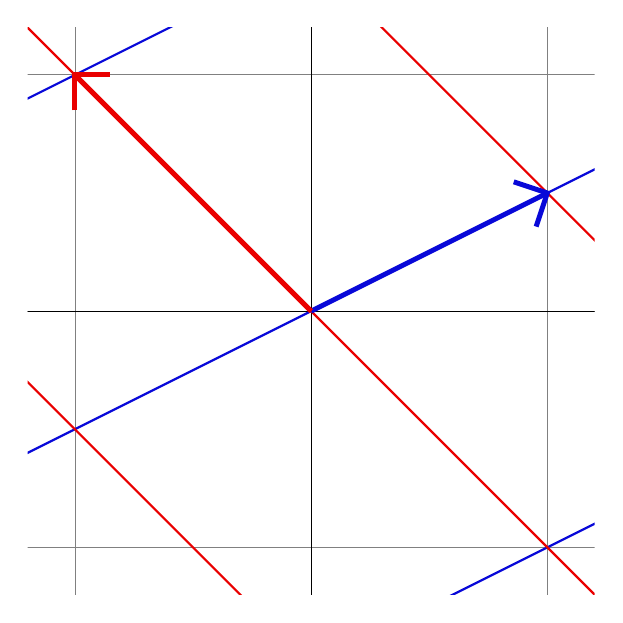
\begin{tikzpicture}[scale=3]
	\definecolor{cBackgroundGrid}{HTML}{808080}
	\definecolor{cBackgroundAxes}{HTML}{000000}
	\definecolor{cI}{HTML}{0808D8}
	\definecolor{cJ}{HTML}{E90000}

	\clip (-1.2,-1.2) rectangle (1.2,1.2);

	\draw[cBackgroundGrid, line width=0.3] (-1.5,-1.5) grid[step=1] (1.5,1.5);
	\draw[cBackgroundAxes] (0,1.5) -- (0,-1.5) (-1.5,0) -- (1.5,0);

	\draw[cI, line width=0.8] (0,-1.5) +(26.565:2) -- +(26.565:-4);
	\draw[cI, line width=0.8] (0,0) +(26.565:2) -- +(26.565:-4);
	\draw[cI, line width=0.8] (0,1.5) +(26.565:2) -- +(26.565:-4);

	\draw[cJ, line width=0.8] (-2,2) -- (2,-2);
	\draw[cJ, line width=0.8] (-2,3.5) -- (2,-0.5);
	\draw[cJ, line width=0.8] (-2,0.5) -- (2,-3.5);

	\draw[cI, line width=1.8] (0,0) -- (1,0.5);
	\draw[cI, line width=1.8] (1,0.5) +(251.565:0.15) -- (1,0.5) -- +(161.565:0.15);

	\draw[cJ, line width=1.8] (0,0) -- (-1,1);
	\draw[cJ, line width=1.8] (-1,0.85) -- (-1,1) -- (-0.85,1);
\end{tikzpicture}

\end{document}
